\documentclass[12pt,oneside,openary]{article}
\usepackage{graphicx}                                                                                                                                          
%\usepackage[dvipdfmx]{graphicx}
%\usepackage{enumerate}
%\usepackage{mediabb}                                                                                                                                            
%\usepackage{amssymb}
%\usepackage{epstopdf}
%\usepackage{ascmac}
%\usepackage{float}
%\usepackage{breqn}
%\usepackage{comment}
%\usepackage{hyperref}
%\usepackage{framed}
%\usepackage{color}
\usepackage{amsmath}
\usepackage{fullpage}
%\usepackage{here}
%\usepackage{fancyhdr}
%\usepackage{lineno}
%\pagestyle{fancyplain}

\begin{document}
\title{Derivation of Angle Dependence in Boost and Rotation}
\author{Theo Koblesky}
\maketitle
%\email{s1420259@u.tsukuba.ac.jp}                                                                                                                                
%\linenumbers

%\begin{equation}
For this derivation, I am using the natural units system (c = 1). For this case we have 2 protons with 100 GeV colliding nearly head on.
\begin{equation}
p^{blue} = \left(\sqrt{100^2+m_{proton}^2},100\sin(\theta^{blue}),0,100\cos(\theta^{blue})\right) 
\end{equation}
\begin{equation}
p^{yellow} = \left(\sqrt{100^2+m_{proton}^2},100 \sin(\theta^{yellow}+\pi),0,100 \cos(\theta^{yellow}+\pi)\right) 
\end{equation}

\begin{figure}[h!]
\begin{center}
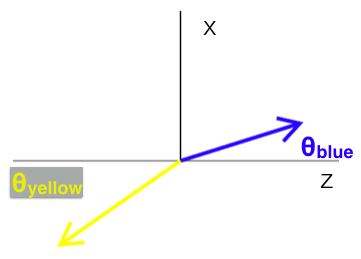
\includegraphics[width=0.45\linewidth]{vector_diagram.png}
\caption{The vector diagram for the blue and yellow 4 momentum vectors.}
\label{fig:diagram2}
\end{center}
\end{figure}

Assuming $\theta^{blue} $ and $\theta^{yellow}$ are small (dropping $\theta^2 order$), we can reduce these components to
\begin{equation}
p^{blue} = \left(\sqrt{100^2+m_{proton}^2},100  \theta^{blue},0,100)\right) 
\end{equation}
\begin{equation}
p^{yellow} = \left(\sqrt{100^2+m_{proton}^2},-100  \theta^{yellow},0,-100\right).
\end{equation}
The total momentum vector is
\begin{equation}
p^{CMS} = (p^{blue}+p^{yellow}).
\end{equation}
From this, we calculate the boost velocity vector to be
\begin{equation}
v^{B} = (p^{CMS}_x,0,0)/E^{CMS}.
\end{equation}
Using the small angle approximation and small mass limit, we obtain
\begin{equation}
v^{B}_x  = \frac{100(\theta^{blue}-\theta^{yellow})}{2\sqrt{100^2+m_{proton}^2}}\approx 0.5(\theta^{blue}-\theta^{yellow}).
\end{equation}
The resulting boost matrix (for the x-direction) is
\[
B=
\begin{bmatrix}
    \gamma & -\gamma v^B_{x} & 0  & 0 \\
    -\gamma v^{B}_x & 1+(\gamma-1) & 0  & 0\\
    0 & 0 & 1 & 0 \\
    0 & 0 & 0  & 1
\end{bmatrix}.
\]
For a given 4 momentum vector of a single particle, we have
\begin{equation}
p = (E,p_x,p_y,p_z).
\end{equation}
The momentum in the boosted frame (in the limit that $\gamma$ $\approx$ 1) is
\begin{equation}
p_{x}\prime=-\gamma v^{B}_x E+p_x\approx -v^{B}_x E+p_x
\end{equation}
\begin{equation}
p_{z}\prime \approx p_z.
\end{equation}
The rotation angle after the boost (assuming $p_z\prime$ $>>$ $p_x\prime$) is
\begin{equation}
\theta_{xz}=\arctan\left(\frac{p^{blue}_x\prime}{p^{blue}_z\prime}\right)\approx \frac{p^{blue}_x\prime}{p^{blue}_z\prime}.
\end{equation}
The resulting rotation matrix is
\[
R=
\begin{pmatrix}
    \cos(\theta_{xz})  & -\sin(\theta_{xz}) \\
     \sin(\theta_{xz})  & \cos(\theta_{xz})
\end{pmatrix}.
\]
The momentum in the rotated frame is
\begin{equation}
p_{x}\prime\prime = p_{x}\prime \cos(\theta_{xz})- p_{z}\prime \sin(\theta_{xz})\approx p_{x}\prime - p_z\prime \theta_{xz}.
\end{equation}
Rewriting $p_x\prime$ in terms of the unprimed momentum we get
\begin{equation}
p_{x}\prime\prime = p_{x} - E v^{B}_x - p_z \frac{p^{blue}_x - E^{blue} v^{B}_x}{p^{blue}_z}
\end{equation}
and then rewriting the boost velocity in terms of the beam angle, we obtain
\begin{equation}
p_{x}\prime\prime = p_{x} - 0.5 E (\theta^{blue}-\theta^{yellow}) - \left(\frac{p_z p^{blue}_x}{p^{blue}_z}\right)+\frac{0.5 p_{z}E^{blue}(\theta^{blue}-\theta^{yellow})}{p^{blue}_z}.
\end{equation}
Using the approximations $p^{blue}_x/p^{blue}_z \approx \theta^{blue}$ and $E^{blue}/p^{blue}_z \approx 1$,
we obtain
\begin{equation}
p_{x}\prime\prime = p_{x} -  0.5E(\theta^{blue}-\theta^{yellow}) - (p_z \theta^{blue})+0.5 p_{z} (\theta^{blue}-\theta^{yellow}).
\end{equation}
If we define $F_{Blue} = 0.5(E+p_z)$
and 
$F_{Yellow} = 0.5(E-p_z)$,
we obtain
\begin{equation}
p_{x}\prime\prime = p_{x} -\theta_{Blue}F_{Blue} - \theta_{Yellow}F_{Yellow}.
\end{equation}

\begin{itemize}
\item For a charged pion at $\eta$ = -3.5 (average BBCs detector location) with $p_T$ = 250 MeV, $E$ = 4.14 GeV and $p_z$ = -4.13 GeV/c, we get the numerical results
$F_{Blue} = 0.00495$
and 
$F_{Yellow} = -4.14$.


\item For a charged pion at $\eta$ = -1.5 (average FVTXs location) with $p_T$ = 250 MeV, $E$ = 0.604 GeV and $p_z$  = -0.532 GeV/c, we get the numerical results
$F_{Blue} =0.036$
and 
$F_{Yellow} = -0.57$.


\item For a charged pion at $\eta$ = 0 (average central arm location) with $p_T$ = 250 MeV, $E$ = 0.286 GeV and $p_z$  = 0.0 GeV/c, we get the numerical results
$F_{Blue} =0.143$
and 
$F_{Yellow} = -0.143$.
\end{itemize}
\begin{figure}[h!]
\begin{center}
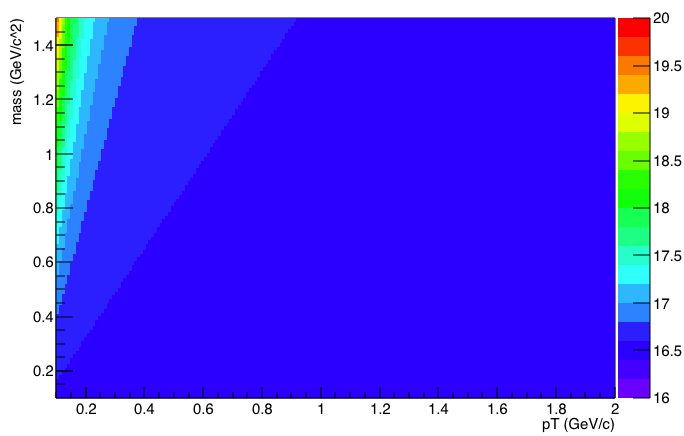
\includegraphics[width=0.75\linewidth]{pt_mass_dep_coeff.png}
\caption{Diagram showing the relevant beam angles. The z-axis is $F_{yellow}$/$p_T$ for a particle with $\eta$ = -3.5}
\label{fig:diagram1}
\end{center}
\end{figure}

%We can set up the equivalent rotation using the yellow beam:
%\begin{equation}
%\theta_{xz}=ATan(\frac{p_{Yellowx}\prime}{p_{Yellowz}\prime})\approx \frac{p_{Yellowx}\prime}{p_{Yellowz}\prime}
%\end{equation}
%\[
%R=
%\begin{pmatrix}
 %   Cos(\theta_{xz})  & Sin(\theta_{xz}) \\
  %   -Sin(\theta_{xz})  & Cos(\theta_{xz})
%\end{pmatrix}
%\]
%\begin{equation}
%p_{x}\prime\prime = p_{x}\prime Cos(\theta_{xz}) +p_{z}\prime Sin(\theta_{xz})\approx p_{x}\prime + p_z\prime \theta_{xz}
%\end{equation}
%\begin{equation}
%p_{z}\prime\prime = -p_{x}\prime Sin(\theta_{xz})+ p_{z}\prime Cos(\theta_{xz})\approx -p_{x}\prime \theta_{xz} + p_z\prime 
%\end{equation}

\end{document}

%%
%% End of file `nppp-template.tex'. 

% LocalWords:  NN
